\documentclass{article}
\usepackage{graphicx}
\usepackage{geometry}
\usepackage{amsmath}
\usepackage{float}
\usepackage{xcolor}
\usepackage{listings}
\usepackage{caption}
\usepackage{subcaption}
\usepackage{xparse}
\usepackage{hyperref}
\usepackage{amssymb}
\usepackage{verbatim}
\usepackage{fancyhdr}
\pagestyle{fancy}
\usepackage{xspace}
\cfoot{}
\lfoot{Università degli Studi di Padova, Laboratorio di Microelettronica, AA 2022-2023}
\rfoot{\thepage}

%\hypersetup{
%    colorlinks=true,
%    linkcolor=blue,
%    filecolor=magenta,      
%    urlcolor=cyan,
%    pdftitle={Overleaf Example},
%    pdfpagemode=FullScreen,
%    }

\usepackage{listings}
 %%%%%%%%%%%%%%%%%%%%%%%%%%%%%%%%%%%%%%%%%%%%%%%%%%%%%%%%%%%%%%%%%%%%%%%%%%%%%%%% 
%%% ~ Arduino Language - Arduino IDE Colors ~                                  %%%
%%%                                                                            %%%
%%% Kyle Rocha-Brownell | 10/2/2017 | No Licence                               %%%
%%% -------------------------------------------------------------------------- %%%
%%%                                                                            %%%
%%% Place this file in your working directory (next to the latex file you're   %%%
%%% working on).  To add it to your project, place:                            %%%
%%%     %%%%%%%%%%%%%%%%%%%%%%%%%%%%%%%%%%%%%%%%%%%%%%%%%%%%%%%%%%%%%%%%%%%%%%%%%%%%%%%% 
%%% ~ Arduino Language - Arduino IDE Colors ~                                  %%%
%%%                                                                            %%%
%%% Kyle Rocha-Brownell | 10/2/2017 | No Licence                               %%%
%%% -------------------------------------------------------------------------- %%%
%%%                                                                            %%%
%%% Place this file in your working directory (next to the latex file you're   %%%
%%% working on).  To add it to your project, place:                            %%%
%%%     %%%%%%%%%%%%%%%%%%%%%%%%%%%%%%%%%%%%%%%%%%%%%%%%%%%%%%%%%%%%%%%%%%%%%%%%%%%%%%%% 
%%% ~ Arduino Language - Arduino IDE Colors ~                                  %%%
%%%                                                                            %%%
%%% Kyle Rocha-Brownell | 10/2/2017 | No Licence                               %%%
%%% -------------------------------------------------------------------------- %%%
%%%                                                                            %%%
%%% Place this file in your working directory (next to the latex file you're   %%%
%%% working on).  To add it to your project, place:                            %%%
%%%    \input{arduinoLanguage.tex}                                             %%%
%%% somewhere before \begin{document} in your latex file.                      %%%
%%%                                                                            %%%
%%% In your document, place your arduino code between:                         %%%
%%%   \begin{lstlisting}[language=Arduino]                                     %%%
%%% and:                                                                       %%%
%%%   \end{lstlisting}                                                         %%%
%%%                                                                            %%%
%%% Or create your own style to add non-built-in functions and variables.      %%%
%%%                                                                            %%%
 %%%%%%%%%%%%%%%%%%%%%%%%%%%%%%%%%%%%%%%%%%%%%%%%%%%%%%%%%%%%%%%%%%%%%%%%%%%%%%%% 

\usepackage{color}
\usepackage{listings}    
\usepackage{courier}

%%% Define Custom IDE Colors %%%
\definecolor{arduinoGreen}    {rgb} {0.17, 0.43, 0.01}
\definecolor{arduinoGrey}     {rgb} {0.47, 0.47, 0.33}
\definecolor{arduinoOrange}   {rgb} {0.8 , 0.4 , 0   }
\definecolor{arduinoBlue}     {rgb} {0.01, 0.61, 0.98}
\definecolor{arduinoDarkBlue} {rgb} {0.0 , 0.2 , 0.5 }

%%% Define Arduino Language %%%
\lstdefinelanguage{Arduino}{
  language=C++, % begin with default C++ settings 
%
%
  %%% Keyword Color Group 1 %%%  (called KEYWORD3 by arduino)
  keywordstyle=\color{arduinoGreen},   
  deletekeywords={  % remove all arduino keywords that might be in c++
                break, case, override, final, continue, default, do, else, for, 
                if, return, goto, switch, throw, try, while, setup, loop, export, 
                not, or, and, xor, include, define, elif, else, error, if, ifdef, 
                ifndef, pragma, warning,
                HIGH, LOW, INPUT, INPUT_PULLUP, OUTPUT, DEC, BIN, HEX, OCT, PI, 
                HALF_PI, TWO_PI, LSBFIRST, MSBFIRST, CHANGE, FALLING, RISING, 
                DEFAULT, EXTERNAL, INTERNAL, INTERNAL1V1, INTERNAL2V56, LED_BUILTIN, 
                LED_BUILTIN_RX, LED_BUILTIN_TX, DIGITAL_MESSAGE, FIRMATA_STRING, 
                ANALOG_MESSAGE, REPORT_DIGITAL, REPORT_ANALOG, SET_PIN_MODE, 
                SYSTEM_RESET, SYSEX_START, auto, int8_t, int16_t, int32_t, int64_t, 
                uint8_t, uint16_t, uint32_t, uint64_t, char16_t, char32_t, operator, 
                enum, delete, bool, boolean, byte, char, const, false, float, double, 
                null, NULL, int, long, new, private, protected, public, short, 
                signed, static, volatile, String, void, true, unsigned, word, array, 
                sizeof, dynamic_cast, typedef, const_cast, struct, static_cast, union, 
                friend, extern, class, reinterpret_cast, register, explicit, inline, 
                _Bool, complex, _Complex, _Imaginary, atomic_bool, atomic_char, 
                atomic_schar, atomic_uchar, atomic_short, atomic_ushort, atomic_int, 
                atomic_uint, atomic_long, atomic_ulong, atomic_llong, atomic_ullong, 
                virtual, PROGMEM,
                Serial, Serial1, Serial2, Serial3, SerialUSB, Keyboard, Mouse,
                abs, acos, asin, atan, atan2, ceil, constrain, cos, degrees, exp, 
                floor, log, map, max, min, radians, random, randomSeed, round, sin, 
                sq, sqrt, tan, pow, bitRead, bitWrite, bitSet, bitClear, bit, 
                highByte, lowByte, analogReference, analogRead, 
                analogReadResolution, analogWrite, analogWriteResolution, 
                attachInterrupt, detachInterrupt, digitalPinToInterrupt, delay, 
                delayMicroseconds, digitalWrite, digitalRead, interrupts, millis, 
                micros, noInterrupts, noTone, pinMode, pulseIn, pulseInLong, shiftIn, 
                shiftOut, tone, yield, Stream, begin, end, peek, read, print, 
                println, available, availableForWrite, flush, setTimeout, find, 
                findUntil, parseInt, parseFloat, readBytes, readBytesUntil, readString, 
                readStringUntil, trim, toUpperCase, toLowerCase, charAt, compareTo, 
                concat, endsWith, startsWith, equals, equalsIgnoreCase, getBytes, 
                indexOf, lastIndexOf, length, replace, setCharAt, substring, 
                toCharArray, toInt, press, release, releaseAll, accept, click, move, 
                isPressed, isAlphaNumeric, isAlpha, isAscii, isWhitespace, isControl, 
                isDigit, isGraph, isLowerCase, isPrintable, isPunct, isSpace, 
                isUpperCase, isHexadecimalDigit, 
                }, 
  morekeywords={   % add arduino structures to group 1
                break, case, override, final, continue, default, do, else, for, 
                if, return, goto, switch, throw, try, while, setup, loop, export, 
                not, or, and, xor, include, define, elif, else, error, if, ifdef, 
                ifndef, pragma, warning,
                }, 
% 
%
  %%% Keyword Color Group 2 %%%  (called LITERAL1 by arduino)
  keywordstyle=[2]\color{arduinoBlue},   
  keywords=[2]{   % add variables and dataTypes as 2nd group  
                HIGH, LOW, INPUT, INPUT_PULLUP, OUTPUT, DEC, BIN, HEX, OCT, PI, 
                HALF_PI, TWO_PI, LSBFIRST, MSBFIRST, CHANGE, FALLING, RISING, 
                DEFAULT, EXTERNAL, INTERNAL, INTERNAL1V1, INTERNAL2V56, LED_BUILTIN, 
                LED_BUILTIN_RX, LED_BUILTIN_TX, DIGITAL_MESSAGE, FIRMATA_STRING, 
                ANALOG_MESSAGE, REPORT_DIGITAL, REPORT_ANALOG, SET_PIN_MODE, 
                SYSTEM_RESET, SYSEX_START, auto, int8_t, int16_t, int32_t, int64_t, 
                uint8_t, uint16_t, uint32_t, uint64_t, char16_t, char32_t, operator, 
                enum, delete, bool, boolean, byte, char, const, false, float, double, 
                null, NULL, int, long, new, private, protected, public, short, 
                signed, static, volatile, String, void, true, unsigned, word, array, 
                sizeof, dynamic_cast, typedef, const_cast, struct, static_cast, union, 
                friend, extern, class, reinterpret_cast, register, explicit, inline, 
                _Bool, complex, _Complex, _Imaginary, atomic_bool, atomic_char, 
                atomic_schar, atomic_uchar, atomic_short, atomic_ushort, atomic_int, 
                atomic_uint, atomic_long, atomic_ulong, atomic_llong, atomic_ullong, 
                virtual, PROGMEM,
                },  
% 
%
  %%% Keyword Color Group 3 %%%  (called KEYWORD1 by arduino)
  keywordstyle=[3]\bfseries\color{arduinoOrange},
  keywords=[3]{  % add built-in functions as a 3rd group
                Serial, Serial1, Serial2, Serial3, SerialUSB, Keyboard, Mouse,
                },      
%
%
  %%% Keyword Color Group 4 %%%  (called KEYWORD2 by arduino)
  keywordstyle=[4]\color{arduinoOrange},
  keywords=[4]{  % add more built-in functions as a 4th group
                abs, acos, asin, atan, atan2, ceil, constrain, cos, degrees, exp, 
                floor, log, map, max, min, radians, random, randomSeed, round, sin, 
                sq, sqrt, tan, pow, bitRead, bitWrite, bitSet, bitClear, bit, 
                highByte, lowByte, analogReference, analogRead, 
                analogReadResolution, analogWrite, analogWriteResolution, 
                attachInterrupt, detachInterrupt, digitalPinToInterrupt, delay, 
                delayMicroseconds, digitalWrite, digitalRead, interrupts, millis, 
                micros, noInterrupts, noTone, pinMode, pulseIn, pulseInLong, shiftIn, 
                shiftOut, tone, yield, Stream, begin, end, peek, read, print, 
                println, available, availableForWrite, flush, setTimeout, find, 
                findUntil, parseInt, parseFloat, readBytes, readBytesUntil, readString, 
                readStringUntil, trim, toUpperCase, toLowerCase, charAt, compareTo, 
                concat, endsWith, startsWith, equals, equalsIgnoreCase, getBytes, 
                indexOf, lastIndexOf, length, replace, setCharAt, substring, 
                toCharArray, toInt, press, release, releaseAll, accept, click, move, 
                isPressed, isAlphaNumeric, isAlpha, isAscii, isWhitespace, isControl, 
                isDigit, isGraph, isLowerCase, isPrintable, isPunct, isSpace, 
                isUpperCase, isHexadecimalDigit, 
                },      
%
%
  %%% Set Other Colors %%%
  stringstyle=\color{arduinoDarkBlue},    
  commentstyle=\color{arduinoGrey},    
%          
%   
  %%%% Line Numbering %%%%
   numbers=left,                    
  numbersep=5pt,                   
  numberstyle=\color{arduinoGrey},    
  %stepnumber=2,                      % show every 2 line numbers
%
%
  %%%% Code Box Style %%%%
  breaklines=true,                    % wordwrapping
  frame=shadowbox,
  tabsize=2,         
  basicstyle=\ttfamily  
}                                             %%%
%%% somewhere before \begin{document} in your latex file.                      %%%
%%%                                                                            %%%
%%% In your document, place your arduino code between:                         %%%
%%%   \begin{lstlisting}[language=Arduino]                                     %%%
%%% and:                                                                       %%%
%%%   \end{lstlisting}                                                         %%%
%%%                                                                            %%%
%%% Or create your own style to add non-built-in functions and variables.      %%%
%%%                                                                            %%%
 %%%%%%%%%%%%%%%%%%%%%%%%%%%%%%%%%%%%%%%%%%%%%%%%%%%%%%%%%%%%%%%%%%%%%%%%%%%%%%%% 

\usepackage{color}
\usepackage{listings}    
\usepackage{courier}

%%% Define Custom IDE Colors %%%
\definecolor{arduinoGreen}    {rgb} {0.17, 0.43, 0.01}
\definecolor{arduinoGrey}     {rgb} {0.47, 0.47, 0.33}
\definecolor{arduinoOrange}   {rgb} {0.8 , 0.4 , 0   }
\definecolor{arduinoBlue}     {rgb} {0.01, 0.61, 0.98}
\definecolor{arduinoDarkBlue} {rgb} {0.0 , 0.2 , 0.5 }

%%% Define Arduino Language %%%
\lstdefinelanguage{Arduino}{
  language=C++, % begin with default C++ settings 
%
%
  %%% Keyword Color Group 1 %%%  (called KEYWORD3 by arduino)
  keywordstyle=\color{arduinoGreen},   
  deletekeywords={  % remove all arduino keywords that might be in c++
                break, case, override, final, continue, default, do, else, for, 
                if, return, goto, switch, throw, try, while, setup, loop, export, 
                not, or, and, xor, include, define, elif, else, error, if, ifdef, 
                ifndef, pragma, warning,
                HIGH, LOW, INPUT, INPUT_PULLUP, OUTPUT, DEC, BIN, HEX, OCT, PI, 
                HALF_PI, TWO_PI, LSBFIRST, MSBFIRST, CHANGE, FALLING, RISING, 
                DEFAULT, EXTERNAL, INTERNAL, INTERNAL1V1, INTERNAL2V56, LED_BUILTIN, 
                LED_BUILTIN_RX, LED_BUILTIN_TX, DIGITAL_MESSAGE, FIRMATA_STRING, 
                ANALOG_MESSAGE, REPORT_DIGITAL, REPORT_ANALOG, SET_PIN_MODE, 
                SYSTEM_RESET, SYSEX_START, auto, int8_t, int16_t, int32_t, int64_t, 
                uint8_t, uint16_t, uint32_t, uint64_t, char16_t, char32_t, operator, 
                enum, delete, bool, boolean, byte, char, const, false, float, double, 
                null, NULL, int, long, new, private, protected, public, short, 
                signed, static, volatile, String, void, true, unsigned, word, array, 
                sizeof, dynamic_cast, typedef, const_cast, struct, static_cast, union, 
                friend, extern, class, reinterpret_cast, register, explicit, inline, 
                _Bool, complex, _Complex, _Imaginary, atomic_bool, atomic_char, 
                atomic_schar, atomic_uchar, atomic_short, atomic_ushort, atomic_int, 
                atomic_uint, atomic_long, atomic_ulong, atomic_llong, atomic_ullong, 
                virtual, PROGMEM,
                Serial, Serial1, Serial2, Serial3, SerialUSB, Keyboard, Mouse,
                abs, acos, asin, atan, atan2, ceil, constrain, cos, degrees, exp, 
                floor, log, map, max, min, radians, random, randomSeed, round, sin, 
                sq, sqrt, tan, pow, bitRead, bitWrite, bitSet, bitClear, bit, 
                highByte, lowByte, analogReference, analogRead, 
                analogReadResolution, analogWrite, analogWriteResolution, 
                attachInterrupt, detachInterrupt, digitalPinToInterrupt, delay, 
                delayMicroseconds, digitalWrite, digitalRead, interrupts, millis, 
                micros, noInterrupts, noTone, pinMode, pulseIn, pulseInLong, shiftIn, 
                shiftOut, tone, yield, Stream, begin, end, peek, read, print, 
                println, available, availableForWrite, flush, setTimeout, find, 
                findUntil, parseInt, parseFloat, readBytes, readBytesUntil, readString, 
                readStringUntil, trim, toUpperCase, toLowerCase, charAt, compareTo, 
                concat, endsWith, startsWith, equals, equalsIgnoreCase, getBytes, 
                indexOf, lastIndexOf, length, replace, setCharAt, substring, 
                toCharArray, toInt, press, release, releaseAll, accept, click, move, 
                isPressed, isAlphaNumeric, isAlpha, isAscii, isWhitespace, isControl, 
                isDigit, isGraph, isLowerCase, isPrintable, isPunct, isSpace, 
                isUpperCase, isHexadecimalDigit, 
                }, 
  morekeywords={   % add arduino structures to group 1
                break, case, override, final, continue, default, do, else, for, 
                if, return, goto, switch, throw, try, while, setup, loop, export, 
                not, or, and, xor, include, define, elif, else, error, if, ifdef, 
                ifndef, pragma, warning,
                }, 
% 
%
  %%% Keyword Color Group 2 %%%  (called LITERAL1 by arduino)
  keywordstyle=[2]\color{arduinoBlue},   
  keywords=[2]{   % add variables and dataTypes as 2nd group  
                HIGH, LOW, INPUT, INPUT_PULLUP, OUTPUT, DEC, BIN, HEX, OCT, PI, 
                HALF_PI, TWO_PI, LSBFIRST, MSBFIRST, CHANGE, FALLING, RISING, 
                DEFAULT, EXTERNAL, INTERNAL, INTERNAL1V1, INTERNAL2V56, LED_BUILTIN, 
                LED_BUILTIN_RX, LED_BUILTIN_TX, DIGITAL_MESSAGE, FIRMATA_STRING, 
                ANALOG_MESSAGE, REPORT_DIGITAL, REPORT_ANALOG, SET_PIN_MODE, 
                SYSTEM_RESET, SYSEX_START, auto, int8_t, int16_t, int32_t, int64_t, 
                uint8_t, uint16_t, uint32_t, uint64_t, char16_t, char32_t, operator, 
                enum, delete, bool, boolean, byte, char, const, false, float, double, 
                null, NULL, int, long, new, private, protected, public, short, 
                signed, static, volatile, String, void, true, unsigned, word, array, 
                sizeof, dynamic_cast, typedef, const_cast, struct, static_cast, union, 
                friend, extern, class, reinterpret_cast, register, explicit, inline, 
                _Bool, complex, _Complex, _Imaginary, atomic_bool, atomic_char, 
                atomic_schar, atomic_uchar, atomic_short, atomic_ushort, atomic_int, 
                atomic_uint, atomic_long, atomic_ulong, atomic_llong, atomic_ullong, 
                virtual, PROGMEM,
                },  
% 
%
  %%% Keyword Color Group 3 %%%  (called KEYWORD1 by arduino)
  keywordstyle=[3]\bfseries\color{arduinoOrange},
  keywords=[3]{  % add built-in functions as a 3rd group
                Serial, Serial1, Serial2, Serial3, SerialUSB, Keyboard, Mouse,
                },      
%
%
  %%% Keyword Color Group 4 %%%  (called KEYWORD2 by arduino)
  keywordstyle=[4]\color{arduinoOrange},
  keywords=[4]{  % add more built-in functions as a 4th group
                abs, acos, asin, atan, atan2, ceil, constrain, cos, degrees, exp, 
                floor, log, map, max, min, radians, random, randomSeed, round, sin, 
                sq, sqrt, tan, pow, bitRead, bitWrite, bitSet, bitClear, bit, 
                highByte, lowByte, analogReference, analogRead, 
                analogReadResolution, analogWrite, analogWriteResolution, 
                attachInterrupt, detachInterrupt, digitalPinToInterrupt, delay, 
                delayMicroseconds, digitalWrite, digitalRead, interrupts, millis, 
                micros, noInterrupts, noTone, pinMode, pulseIn, pulseInLong, shiftIn, 
                shiftOut, tone, yield, Stream, begin, end, peek, read, print, 
                println, available, availableForWrite, flush, setTimeout, find, 
                findUntil, parseInt, parseFloat, readBytes, readBytesUntil, readString, 
                readStringUntil, trim, toUpperCase, toLowerCase, charAt, compareTo, 
                concat, endsWith, startsWith, equals, equalsIgnoreCase, getBytes, 
                indexOf, lastIndexOf, length, replace, setCharAt, substring, 
                toCharArray, toInt, press, release, releaseAll, accept, click, move, 
                isPressed, isAlphaNumeric, isAlpha, isAscii, isWhitespace, isControl, 
                isDigit, isGraph, isLowerCase, isPrintable, isPunct, isSpace, 
                isUpperCase, isHexadecimalDigit, 
                },      
%
%
  %%% Set Other Colors %%%
  stringstyle=\color{arduinoDarkBlue},    
  commentstyle=\color{arduinoGrey},    
%          
%   
  %%%% Line Numbering %%%%
   numbers=left,                    
  numbersep=5pt,                   
  numberstyle=\color{arduinoGrey},    
  %stepnumber=2,                      % show every 2 line numbers
%
%
  %%%% Code Box Style %%%%
  breaklines=true,                    % wordwrapping
  frame=shadowbox,
  tabsize=2,         
  basicstyle=\ttfamily  
}                                             %%%
%%% somewhere before \begin{document} in your latex file.                      %%%
%%%                                                                            %%%
%%% In your document, place your arduino code between:                         %%%
%%%   \begin{lstlisting}[language=Arduino]                                     %%%
%%% and:                                                                       %%%
%%%   \end{lstlisting}                                                         %%%
%%%                                                                            %%%
%%% Or create your own style to add non-built-in functions and variables.      %%%
%%%                                                                            %%%
 %%%%%%%%%%%%%%%%%%%%%%%%%%%%%%%%%%%%%%%%%%%%%%%%%%%%%%%%%%%%%%%%%%%%%%%%%%%%%%%% 

\usepackage{color}
\usepackage{listings}    
\usepackage{courier}

%%% Define Custom IDE Colors %%%
\definecolor{arduinoGreen}    {rgb} {0.17, 0.43, 0.01}
\definecolor{arduinoGrey}     {rgb} {0.47, 0.47, 0.33}
\definecolor{arduinoOrange}   {rgb} {0.8 , 0.4 , 0   }
\definecolor{arduinoBlue}     {rgb} {0.01, 0.61, 0.98}
\definecolor{arduinoDarkBlue} {rgb} {0.0 , 0.2 , 0.5 }

%%% Define Arduino Language %%%
\lstdefinelanguage{Arduino}{
  language=C++, % begin with default C++ settings 
%
%
  %%% Keyword Color Group 1 %%%  (called KEYWORD3 by arduino)
  keywordstyle=\color{arduinoGreen},   
  deletekeywords={  % remove all arduino keywords that might be in c++
                break, case, override, final, continue, default, do, else, for, 
                if, return, goto, switch, throw, try, while, setup, loop, export, 
                not, or, and, xor, include, define, elif, else, error, if, ifdef, 
                ifndef, pragma, warning,
                HIGH, LOW, INPUT, INPUT_PULLUP, OUTPUT, DEC, BIN, HEX, OCT, PI, 
                HALF_PI, TWO_PI, LSBFIRST, MSBFIRST, CHANGE, FALLING, RISING, 
                DEFAULT, EXTERNAL, INTERNAL, INTERNAL1V1, INTERNAL2V56, LED_BUILTIN, 
                LED_BUILTIN_RX, LED_BUILTIN_TX, DIGITAL_MESSAGE, FIRMATA_STRING, 
                ANALOG_MESSAGE, REPORT_DIGITAL, REPORT_ANALOG, SET_PIN_MODE, 
                SYSTEM_RESET, SYSEX_START, auto, int8_t, int16_t, int32_t, int64_t, 
                uint8_t, uint16_t, uint32_t, uint64_t, char16_t, char32_t, operator, 
                enum, delete, bool, boolean, byte, char, const, false, float, double, 
                null, NULL, int, long, new, private, protected, public, short, 
                signed, static, volatile, String, void, true, unsigned, word, array, 
                sizeof, dynamic_cast, typedef, const_cast, struct, static_cast, union, 
                friend, extern, class, reinterpret_cast, register, explicit, inline, 
                _Bool, complex, _Complex, _Imaginary, atomic_bool, atomic_char, 
                atomic_schar, atomic_uchar, atomic_short, atomic_ushort, atomic_int, 
                atomic_uint, atomic_long, atomic_ulong, atomic_llong, atomic_ullong, 
                virtual, PROGMEM,
                Serial, Serial1, Serial2, Serial3, SerialUSB, Keyboard, Mouse,
                abs, acos, asin, atan, atan2, ceil, constrain, cos, degrees, exp, 
                floor, log, map, max, min, radians, random, randomSeed, round, sin, 
                sq, sqrt, tan, pow, bitRead, bitWrite, bitSet, bitClear, bit, 
                highByte, lowByte, analogReference, analogRead, 
                analogReadResolution, analogWrite, analogWriteResolution, 
                attachInterrupt, detachInterrupt, digitalPinToInterrupt, delay, 
                delayMicroseconds, digitalWrite, digitalRead, interrupts, millis, 
                micros, noInterrupts, noTone, pinMode, pulseIn, pulseInLong, shiftIn, 
                shiftOut, tone, yield, Stream, begin, end, peek, read, print, 
                println, available, availableForWrite, flush, setTimeout, find, 
                findUntil, parseInt, parseFloat, readBytes, readBytesUntil, readString, 
                readStringUntil, trim, toUpperCase, toLowerCase, charAt, compareTo, 
                concat, endsWith, startsWith, equals, equalsIgnoreCase, getBytes, 
                indexOf, lastIndexOf, length, replace, setCharAt, substring, 
                toCharArray, toInt, press, release, releaseAll, accept, click, move, 
                isPressed, isAlphaNumeric, isAlpha, isAscii, isWhitespace, isControl, 
                isDigit, isGraph, isLowerCase, isPrintable, isPunct, isSpace, 
                isUpperCase, isHexadecimalDigit, 
                }, 
  morekeywords={   % add arduino structures to group 1
                break, case, override, final, continue, default, do, else, for, 
                if, return, goto, switch, throw, try, while, setup, loop, export, 
                not, or, and, xor, include, define, elif, else, error, if, ifdef, 
                ifndef, pragma, warning,
                }, 
% 
%
  %%% Keyword Color Group 2 %%%  (called LITERAL1 by arduino)
  keywordstyle=[2]\color{arduinoBlue},   
  keywords=[2]{   % add variables and dataTypes as 2nd group  
                HIGH, LOW, INPUT, INPUT_PULLUP, OUTPUT, DEC, BIN, HEX, OCT, PI, 
                HALF_PI, TWO_PI, LSBFIRST, MSBFIRST, CHANGE, FALLING, RISING, 
                DEFAULT, EXTERNAL, INTERNAL, INTERNAL1V1, INTERNAL2V56, LED_BUILTIN, 
                LED_BUILTIN_RX, LED_BUILTIN_TX, DIGITAL_MESSAGE, FIRMATA_STRING, 
                ANALOG_MESSAGE, REPORT_DIGITAL, REPORT_ANALOG, SET_PIN_MODE, 
                SYSTEM_RESET, SYSEX_START, auto, int8_t, int16_t, int32_t, int64_t, 
                uint8_t, uint16_t, uint32_t, uint64_t, char16_t, char32_t, operator, 
                enum, delete, bool, boolean, byte, char, const, false, float, double, 
                null, NULL, int, long, new, private, protected, public, short, 
                signed, static, volatile, String, void, true, unsigned, word, array, 
                sizeof, dynamic_cast, typedef, const_cast, struct, static_cast, union, 
                friend, extern, class, reinterpret_cast, register, explicit, inline, 
                _Bool, complex, _Complex, _Imaginary, atomic_bool, atomic_char, 
                atomic_schar, atomic_uchar, atomic_short, atomic_ushort, atomic_int, 
                atomic_uint, atomic_long, atomic_ulong, atomic_llong, atomic_ullong, 
                virtual, PROGMEM,
                },  
% 
%
  %%% Keyword Color Group 3 %%%  (called KEYWORD1 by arduino)
  keywordstyle=[3]\bfseries\color{arduinoOrange},
  keywords=[3]{  % add built-in functions as a 3rd group
                Serial, Serial1, Serial2, Serial3, SerialUSB, Keyboard, Mouse,
                },      
%
%
  %%% Keyword Color Group 4 %%%  (called KEYWORD2 by arduino)
  keywordstyle=[4]\color{arduinoOrange},
  keywords=[4]{  % add more built-in functions as a 4th group
                abs, acos, asin, atan, atan2, ceil, constrain, cos, degrees, exp, 
                floor, log, map, max, min, radians, random, randomSeed, round, sin, 
                sq, sqrt, tan, pow, bitRead, bitWrite, bitSet, bitClear, bit, 
                highByte, lowByte, analogReference, analogRead, 
                analogReadResolution, analogWrite, analogWriteResolution, 
                attachInterrupt, detachInterrupt, digitalPinToInterrupt, delay, 
                delayMicroseconds, digitalWrite, digitalRead, interrupts, millis, 
                micros, noInterrupts, noTone, pinMode, pulseIn, pulseInLong, shiftIn, 
                shiftOut, tone, yield, Stream, begin, end, peek, read, print, 
                println, available, availableForWrite, flush, setTimeout, find, 
                findUntil, parseInt, parseFloat, readBytes, readBytesUntil, readString, 
                readStringUntil, trim, toUpperCase, toLowerCase, charAt, compareTo, 
                concat, endsWith, startsWith, equals, equalsIgnoreCase, getBytes, 
                indexOf, lastIndexOf, length, replace, setCharAt, substring, 
                toCharArray, toInt, press, release, releaseAll, accept, click, move, 
                isPressed, isAlphaNumeric, isAlpha, isAscii, isWhitespace, isControl, 
                isDigit, isGraph, isLowerCase, isPrintable, isPunct, isSpace, 
                isUpperCase, isHexadecimalDigit, 
                },      
%
%
  %%% Set Other Colors %%%
  stringstyle=\color{arduinoDarkBlue},    
  commentstyle=\color{arduinoGrey},    
%          
%   
  %%%% Line Numbering %%%%
   numbers=left,                    
  numbersep=5pt,                   
  numberstyle=\color{arduinoGrey},    
  %stepnumber=2,                      % show every 2 line numbers
%
%
  %%%% Code Box Style %%%%
  breaklines=true,                    % wordwrapping
  frame=shadowbox,
  tabsize=2,         
  basicstyle=\ttfamily  
}

\title{Esperienza di laboratorio\\\textbf{Arduino DUE\\Display LCD e sensori}}
\author{Gruppo A6\\Giacomo Calabria - 2007964\\Daniele Venturini - 1195858}
\date{19 May 2023}

\begin{document}
    \begin{figure}
        \centering
        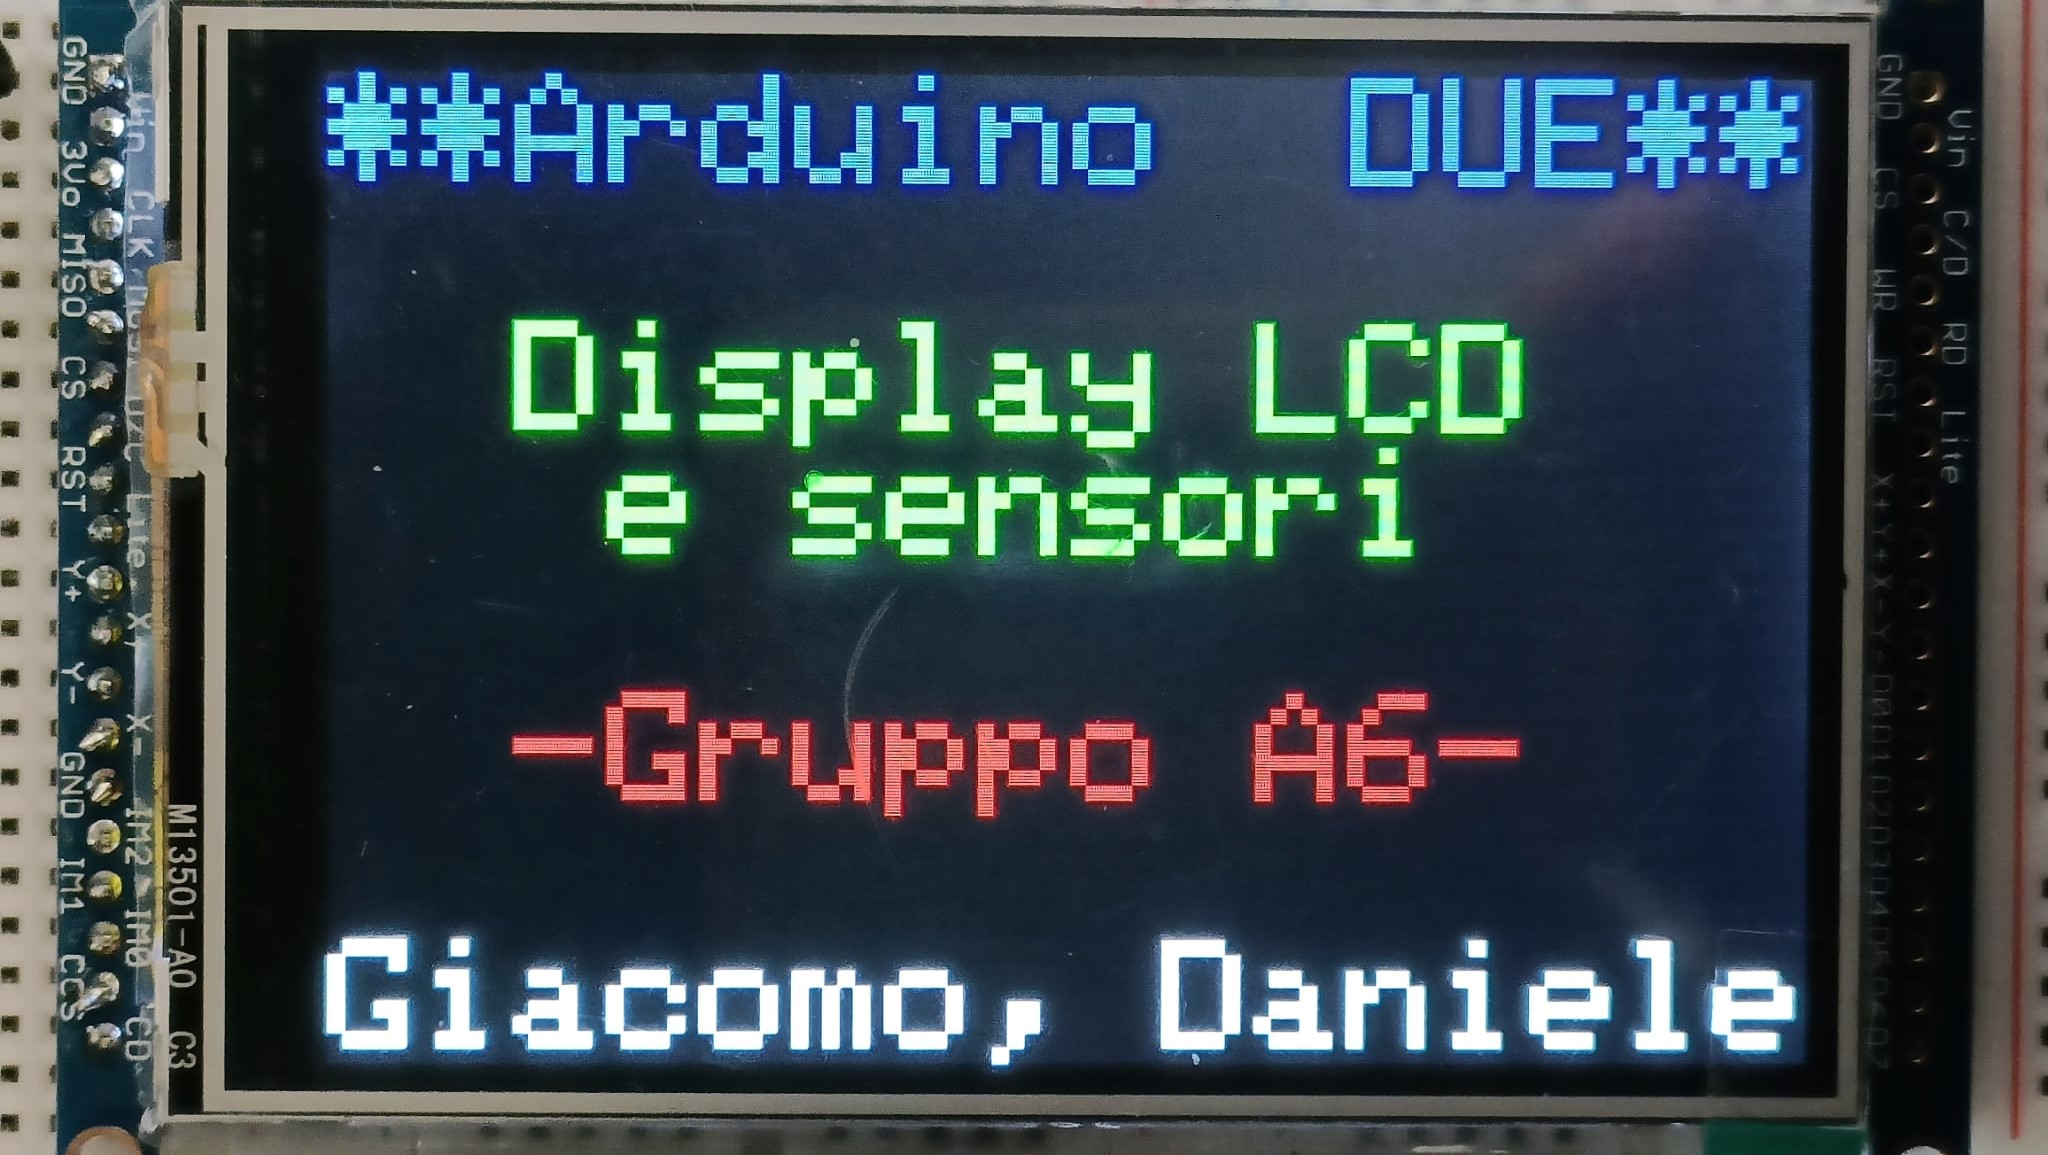
\includegraphics[width=0.75\linewidth]{images/IMG-20230519-WA0006.jpg}
    \end{figure}
    \maketitle
    \tableofcontents
    \clearpage
    
    \section*{INTRODUZIONE}
    Lo scopo dell'esperienza di laboratorio è studiare e valutare mediante misure di laboratorio le proprietà degli stadi di potenza degli amplificatori in classe A e B. Verranno poi valutate le distorsioni di crossover di ciascuno stadio, implementando una metodologia per la riduzione della distorsione di crossover mediante l'uso della retroazione.\\\\
Il circuito realizzato in questa esercitazione è un amplificatore adatto per amplificare il segnale generato da una piccola radio o da un lettore MP3.
\subsection*{Strumentazione necessaria:}
\begin{itemize}
    \item Generatore di forma d'onda arbitraria
    \item Oscilloscopio a 2 canali
    \item Alimentatore da banco
    \item 1 connettore BNC a “T”
	\item 2 connettore BNC maschio/banana femmina
	\item 1 connettore BNC femmina-femmina
	\item 1 cavo BNC
	\item Cavo 1 mm
	\item Spellafili
    \item Lettore MP3
\end{itemize}
    \clearpage
    
    \section{Primo esperimento}
    Il primo esperimento ha lo scopo di introdurre le procedure di comando di un display TFT mediante scheda Arduino DUE. Si scriverà un programma che realizzi un semplice cronometro a tre stati di funzionamento
\begin{itemize}
    \item \textbf{Stato 0:} il circuito attende la pressione del tasto \textit{T} visualizzando il tempo "0.00 s". Durante l'attesa viene visualizzata la scritta "Press to Start"
    \item \textbf{Stato 1:} nel momento in cui il tasto \textit{T} viene premuto, il timer comincia a misurare il tempo, a step di 50 ms. La misura finisce quando il tasto viene rilasciato. Durante la misura appare la scritta “Release to Stop”
    \item \textbf{Stato 2:} quando il tasto T viene rilasciato, il timer si ferma, e visualizza il tempo totale durante cui il tasto è rimasto premuto. Viene inoltre visualizzata la scritta “Press to Reset”. Una ulteriore pressione del tasto \textit{T} resetta il timer e fa tornare il circuito allo stato 0
\end{itemize}
I componenti necessari a questa esperienza sono:
\begin{itemize}
    \item Scheda Arduino DUE
    \item Breadboard e cavi
    \item Display TFT 3.5" 320x480, \textit{HX8357} Adafruit
    \item Interruttore a bottone, FSM2JART, Cod. RS 745-5185
    \item Resistenza $R=10\text{ k}\Omega,0.25\text{ W}$
\end{itemize}
Il circuito è alimentato mediante porta USB del PC, la quale eroga circa $(\sim 5 V)$.
\subsection{Codice}
La libreria \texttt{Adafruit\_HX8357.h}, insieme alle librerie \texttt{Adafruit\_GFX.h} e \texttt{SPI.h} permette alla scheda arduino di comunicare con il Display HX8357 tramite le funzioni dedicate.
\begin{lstlisting}[frame=single, language=Arduino]
#include <SPI.h>
#include "Adafruit_GFX.h"
#include "Adafruit_HX8357.h"

#define TFT_CS 10
#define TFT_DC 9

Adafruit_HX8357 tft = Adafruit_HX8357(TFT_CS, TFT_DC, -1); 
// TFT_RST set to -1 to tie it to Arduino's reset

#define buttonPin 2

int buttonState = LOW;
int lastButtonState = LOW;

unsigned long startTime = 0;

int stato = 0;
int reset = 0;

void setup(){  
  pinMode(buttonPin, INPUT);
  tft.begin();
  tft.setRotation(3);
  tft.fillScreen(HX8357_BLACK);
  tft.setTextColor(HX8357_GREEN);
  tft.setTextSize(8);
  tft.setCursor(100,0);
  tft.println("TIMER");
  tft.setTextColor(HX8357_BLUE);
  tft.setCursor(100, 80);
  tft.print("0.00 s");
  tft.setCursor(20, 180);
  tft.setTextColor(HX8357_RED);
  tft.setTextSize(5);
  tft.print("Press to Start");
}
\end{lstlisting}
\begin{lstlisting}[frame=single, language=Arduino]
void loop() {
  buttonState = digitalRead(buttonPin);
  if(buttonState == HIGH && lastButtonState == LOW && reset == 1){
    startTime = 0;
    reset = 0;
    stato = 0;
    tft.fillRect(0, 60, 480, 320, HX8357_BLACK);
    tft.setTextSize(8);
    tft.setTextColor(HX8357_BLUE);
    tft.setCursor(100, 80);
    tft.print("0.00 s");
    tft.setCursor(20, 180);
    tft.setTextColor(HX8357_RED);
    tft.setTextSize(5);
    tft.print("Press to Start");
  }
\end{lstlisting}
\clearpage
\begin{lstlisting}[frame=single, language=Arduino]
  if (buttonState == HIGH && lastButtonState == LOW && stato == 0){
    lastButtonState = buttonState;
    stato = 1;
    
    if(startTime == 0){
      startTime = millis();
    }
    
    tft.fillRect(0, 60, 480, 320, HX8357_BLACK);
    tft.setCursor(20, 180);
    tft.setTextSize(5);
    tft.setTextColor(HX8357_RED);
    tft.print("Release to Stop");
  }
  if (stato == 1 && buttonState == HIGH){
    unsigned long centiseconds = (millis() - startTime) / 10;
    unsigned long seconds = centiseconds / 100;
    centiseconds %= 100;

    tft.setTextSize(8);
    tft.setTextColor(HX8357_BLUE);
    tft.setCursor(100, 80);
    tft.print(String(seconds));
    tft.print(".");
    if (centiseconds < 10) {
      tft.print("0");
    }
    tft.print(String(centiseconds));
    tft.println(" s");
    delay(50);
    tft.fillRect(0, 60, 480, 80, HX8357_BLACK);
  }
\end{lstlisting}
\clearpage
\begin{lstlisting}[frame=single, language=Arduino]
  if (buttonState == LOW && lastButtonState == HIGH){
    lastButtonState = buttonState;

    tft.fillRect(0, 60, 480, 320, HX8357_BLACK);
    tft.setCursor(20, 180);
    tft.setTextSize(5);
    tft.setTextColor(HX8357_RED);
    tft.print("Press to Reset");

    unsigned long centiseconds = (millis() - startTime) / 10;
    unsigned long seconds = centiseconds / 100;
    centiseconds %= 100;

    tft.setTextSize(8);
    tft.setTextColor(HX8357_BLUE);
    tft.setCursor(100, 80);
    tft.print(String(seconds));
    tft.print(".");
    if (centiseconds < 10) {
      tft.print("0");
    }
    tft.print(String(centiseconds));
    tft.println(" s");
    reset = 1;
    stato = 3;
    startTime = 0;
  }
}
\end{lstlisting}
E' possibile apprezzare il funzionamento del circuito dal video al \href{}{seguente link errato} 
    \clearpage
    
    \section{Secondo esperimento}
    In questo esperimento si vuole costruire e studiare un amplificatore in classe B, realizzato tramite push-pull. Il circuito è riportato in Figura \ref{fig:Circuit2}.
\begin{figure}[H]
    \centering
    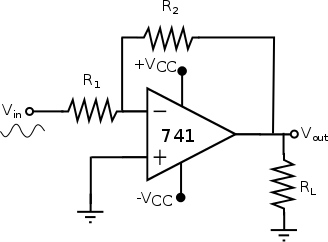
\includegraphics[width=\linewidth]{images/Circuit2.png}
    \caption{Schema circuito}
    \label{fig:Circuit2}
\end{figure}
Il circuito è alimentato dalla tensione duale: $\pm V_{CC}=\pm3V$.\\\\
Il funzionamento per i primi 2 stadi è uguale a quanto detto nel Paragrafo \ref{ch:Spiegazione1}, mentre lo stadio di uscita permette di avere un rendimento migliore di quello ottenuto nell'esperienza precedente. L'efficienza di questo tipo di stadio è dovuta all'attivazione di un solo transistor per semionda. Tuttavia, come si vedrà successivamente, questo circuito ha l'inconveniente di una sensibile distorsione di crossover, dovuta alla soglia di conduzione dei transistor.
\subsection{Assemblaggi e settaggi}
Il circuito in Figura \ref{fig:Circuit2} è stato realizzato modificando direttamente lo schema in classe A (Figura \ref{fig:Circuit1}) con uno stadio in classe B e sostituendo l'integrato MCP6002 con l'integrato TL082CP.\\\\
Lo stadio in classe B push-pull è stato realizzato utilizzando l'accoppiamento di un transistor di potenza NPN $(Q_1)$, codice TIP41CG e un transistor PNP di potenza $(Q_2)$, codice TIP42CG. Le altre componenti sono rimaste invariate dal Primo esperimento\\\\
Il generatore di forma d'onda è stato impostato con il seguente segnale:
\begin{itemize}
    \item Forma d'onda: sinusoidale
    \item Ampiezza iniziale: $100mV$ picco-picco
    \item Frequenza: $330Hz$ (nota Mi)
\end{itemize}
\clearpage
\subsection{Procedura di valutazione e risultati}
Dopo aver acceso l'alimentazione, l'oscilloscopio è stato impostato in modo da visualizzare il segnale di ingresso e il segnale di uscita. Il potenziometro che regola il volume è stato regolato in modo di raggiungere un'ampiezza di $1V_{pp}$ sul segnale di uscita.\\
Si è proseguito a misurare i due segnali con l'oscilloscopio, le cui forme d'onda sono riportare in Figura \ref{fig:scope_9} 
\begin{figure}[H]
    \centering
    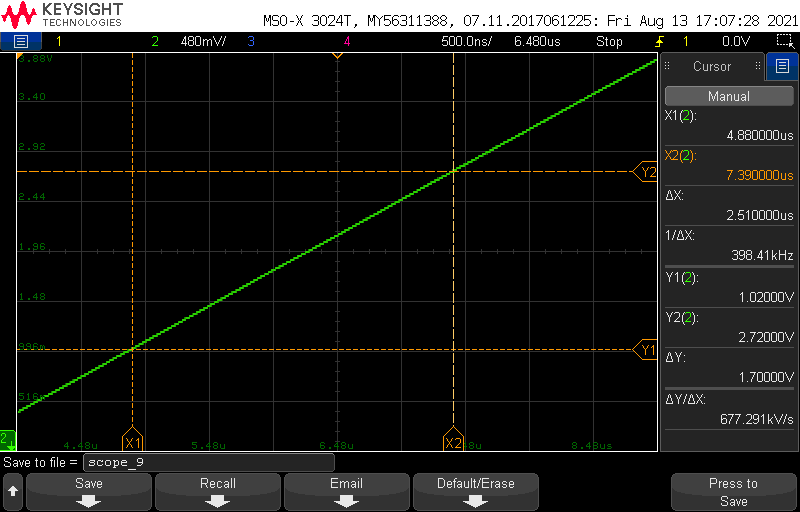
\includegraphics[width=0.7\linewidth]{images/scope_9.png}
    \caption{Segnali di ingresso e uscita dell'amplificatore in classe B}
    \label{fig:scope_9}
\end{figure}
Si è proseguito misurando, attraverso i cursori dell'oscilloscopio, il tempo morto dovuto alla distorsione di crossover.
\begin{equation*}
    \text{Dead time} = 503.125\mu s
\end{equation*}
risultato piùttosto rilevante, considerato che la forma d'onda data in ingresso ha periodo di $T=3\text{ms}$. Si riporta in Figura \ref{fig:scope_11} il dettaglio della distorsione di crossover
\begin{figure}[H]
    \centering
    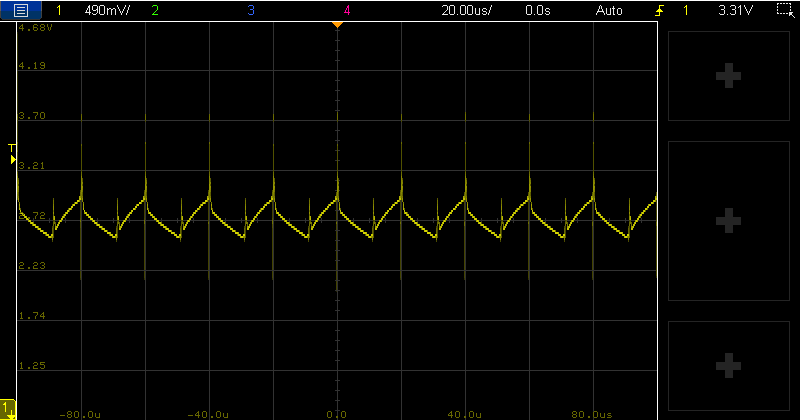
\includegraphics[width=0.7\linewidth]{images/scope_11.png}
    \caption{Dettaglio misurazione distorsione crossover}
    \label{fig:scope_11}
\end{figure}
\subsubsection{Lettore MP3}
Come spiegato nella prima esperienza, si deciso di utilizzare una resistenza di 8$\Omega$ al posto dell'altoparlante, quindi non si è potuto svolgere la prova della riproduzione di una traccia audio. L'obiettivo era quello di sentire l'effetto della distorsione di crossover.
\subsubsection{Commenti}
Le prestazioni di questo amplificatore sono buone, anche se con qualche compromesso. Infatti a livello teorico il rendimento è molto alto, ci sono poce dispersioni di potenza. Come contro, questo circuito ha una distorsione del segnale di uscita decisamente elevata.
    \clearpage
    
    \section{Terzo esperimento}
    In questa esperienza si vuole realizzare un misuratore di distanza utilizzando il sensore di distanza a ultrasuoni HC-SR04, il cui pinout è riportato in Figura \ref{fig:HC-SR04}. Si vuole utilizzare il sensore in modo "nativo", senza utilizzare librerie già scritte. Sono stati utilizzati i seguenti componenti:
\begin{itemize}
    \item Scheda Arduino DUE, breadboard e cavi.
    \item Display TFT 3.5" 320x480, \textit{HX8357} Adafruit
    \item Sensore ultrasonico distanza HC-SR04
\end{itemize}
Il circuito è alimentato mediante porta USB del PC, la quale eroga circa $(\sim 5 V)$. Il sensore HC-SR04 è alimentato con una tensione di $V_{CC}=5$ V. Per garantire la sicurezza degli ingressi della scheda Arduino Due, che operano a una tensione di 3.3 V, si è realizzato un semplice partitore di tensione collegato all'uscita del sensore (ECHO). Il partitore di tensione riduce la tensione di uscita del sensore a un valore prossimo a 3.3 V, consentendo così all'Arduino Due di rilevare correttamente il segnale.
\begin{figure}[H]
    \centering
    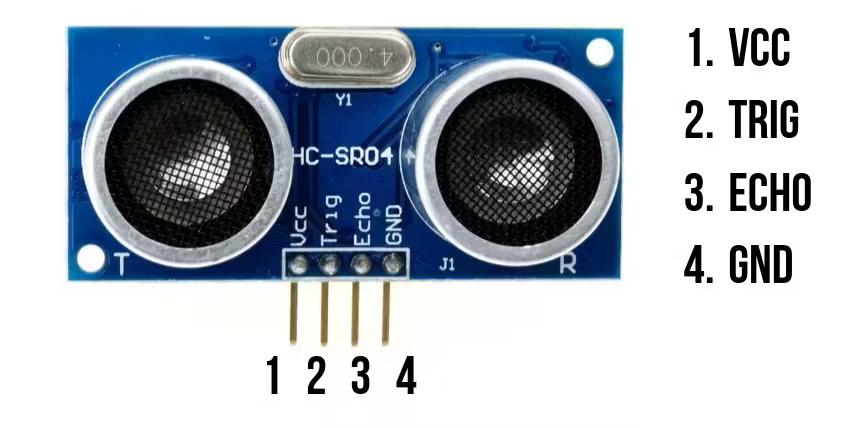
\includegraphics[width=0.5\linewidth]{images/HC-SR04.png}
    \caption{Pinout del sensore HC-SR04}
    \label{fig:HC-SR04}
\end{figure}
\subsection{Codice - Interfaccia grafica}
\begin{lstlisting}[frame=single, language=Arduino]
#include <SPI.h>
#include "Adafruit_GFX.h"
#include "Adafruit_HX8357.h"

#define TRIG_PIN 7
#define ECHO_PIN 6

#define TFT_CS 10
#define TFT_DC 9
Adafruit_HX8357 tft = Adafruit_HX8357(TFT_CS, TFT_DC, -1); 

void setup(){
    pinMode(ECHO_PIN, INPUT);
    pinMode(TRIG_PIN, OUTPUT);
\end{lstlisting}
\begin{lstlisting}[frame=single, language=Arduino]
    // Configurazione del display
    tft.begin();
    tft.setRotation(3);
    tft.fillScreen(HX8357_BLACK);
    tft.setTextColor(HX8357_GREEN);
    tft.setTextSize(6);
    tft.setCursor(60,0);
    tft.println("Distanza");
    tft.setTextColor(HX8357_WHITE);
    tft.setTextSize(10);
}

void loop(){
    String DistTxt = String(distance());
    
    tft.fillRect(0,120,480,320,HX8357_BLACK);
    tft.setCursor(0,150);
    tft.println(DistTxt + " cm");
    
    delay(100);
}
\end{lstlisting}
\subsection{Codice - Lettura sensore HC-SR04}
\begin{lstlisting}[frame=single, language=Arduino]
long distance(){
    long d = 0;
    long duration = 0;
    // Invio dell' inpulso di TRIG
    digitalWrite(TRIG_PIN, LOW);
    delayMicroseconds(2);
    digitalWrite(TRIG_PIN, HIGH);
    delayMicroseconds(2);
    digitalWrite(TRIG_PIN, LOW);
    delayMicroseconds(2);
    // Lettura della durata dell' inpulso da ECHO
    duration = pulseIn(ECHO_PIN, HIGH);
    d = (duration * 100) / 5830;
    delay(25);
    return d;
}
\end{lstlisting}
\clearpage
\noindent La funzione integrata \texttt{pulseIn(pin,value)} ritorna il tempo in microsecondi in cui un determinato \texttt{pin} mantiene il livello \texttt{value}, legge quindi la durata di un inpulso su un pin e ne ritorna la lunghezza in microsecondi. In questo caso fa partire un timer quando il pin \texttt{ECHO\_PIN} commuta a livello \texttt{HIGH} e interrompe il timer quando il pin ritorna a livello \texttt{LOW}, ritornando poi il valore del timer in microsecondi
\begin{figure}[H]
    \centering
    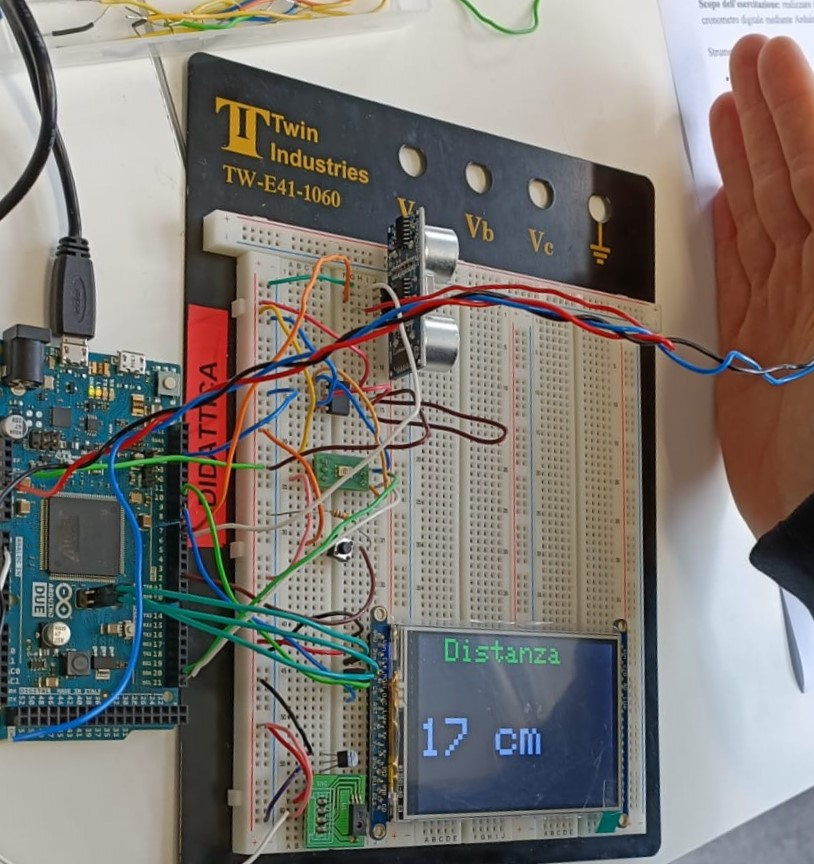
\includegraphics[width=.65\linewidth]{images/IMG-20230519-WA0010.jpg}
    \caption{Prova del funzionamento del sensore}
\end{figure}
\end{document}
